\subsection{\textit{AE-VAL}}
\label{sec:aeval}

\begin{figure}[!t]
\centering
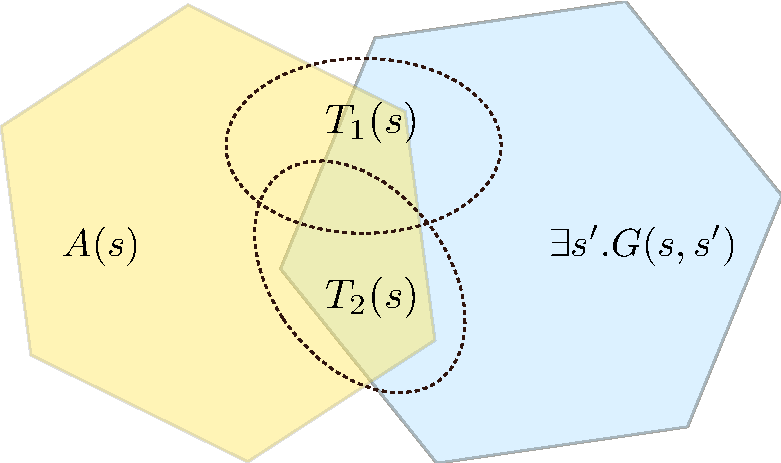
\includegraphics[width=3.5in]{aeval_invalid}
\caption{Region of validity computed for an example requiring \aeval to iterate two times.}
\label{fg:aeval}
\end{figure}

\aeval~\cite{fedyukovich2015automated} is an algorithm to decide validity and extract Skolem functions.
It takes as input a formula of the form $\forall s \,.\,  A(s) \Rightarrow \exists s' . G(s,s')$, 
where $A(s)$ has only existential\andreas{you meant universal here, right?} quantifiers, and $G(s,s')$ is quantifier-free.
%
\andreas{I suppose that the partitions P are the ones named T in the Figure. I think we should keep the same name or the reader might get confused.}
While deciding the validity, \aeval iteratively enumerates models of $A(s) \land G (s, s')$ and groups them into a set of partitions $\{P_i(s)\}$, such that each $P_i(s) \Rightarrow \exists s' . G (s, s')$.
We say that after $n$ iterations, \aeval establishes a formula $R_n(s) \eqdef \bigvee_{i=1}^n P_i(s)$ which is by definition an under-approximation of $\exists s' . G (s, s')$.

If after $n$ iterations, it happens that $A(s) \Rightarrow R_n(s)$ then $\forall s \,.\,  A(s) \Rightarrow \exists s' . G(s,s')$ is valid, and \aeval generates a Skolem function as described in~\cite{katis2016synthesis}.
Alternatively, if $A(s) \land  G (s, s') \land \neg{R_n (s, s')}$ is unsatisfiable, then $A(s) \land \neg G (s, s')$ is satisfiable, or equivalently $\forall s \,.\,  A(s) \Rightarrow \exists s' . G(s,s')$ is invalid (see an example in Figure~\ref{fg:aeval}).
In both cases, we say that $A(s) \land R_n(s)$ is a \emph{region of validity}, meaning that $\forall s \,.\,  A(s) \land R_n(s) \Rightarrow \exists s' . G(s,s')$ is valid by construction.

\begin{lemma}
If formula $\forall s \,.\,  A(s) \Rightarrow \exists s' . G(s,s')$ is invalid, and $A(s) \land R_n(s)$ is the region of validity, then there is no other formula $S(s)$ such that $A(s) \land R_n(s) \Rightarrow S(s)$ and $\forall s \,.\,  S(s) \Rightarrow \exists s' . G(s,s')$.

\label{lem:subset}
\end{lemma}
